%%%%%%%%%%%%%%%%%%%%%%%%%%%%%%%%%%%%%%%%%%%%%%%%%%%%%%%%%%%%%%%
% Welcome to the MAT320 Homework template on Overleaf -- just edit your
% LaTeX on the left, and we'll compile it for you on the right.
%%%%%%%%%%%%%%%%%%%%%%%%%%%%%%%%%%%%%%%%%%%%%%%%%%%%%%%%%%%%%%%
% --------------------------------------------------------------
% Based on a homework template by Dana Ernst.
% --------------------------------------------------------------
% This is all preamble stuff that you don't have to worry about.
% Head down to where it says "Start here"
% --------------------------------------------------------------

\documentclass[12pt]{article}

\usepackage{graphicx}
\graphicspath{{./images/}}
\usepackage{textcomp} % cent symbol, such as \textcent
\usepackage[margin=1in]{geometry} 
\usepackage{amsmath,amsthm,amssymb}
\usepackage{mathtools} % ceiling function
\DeclarePairedDelimiter{\ceil}{\lceil}{\rceil}
% https://tex.stackexchange.com/questions/146306/how-to-make-horizontal-lists
\usepackage[inline]{enumitem} % allows using letters in enumerate list environment

% source: https://stackoverflow.com/questions/3175105/inserting-code-in-this-latex-document-with-indentation

\usepackage{listings}
\usepackage{color}

\definecolor{dkgreen}{rgb}{0,0.6,0}
\definecolor{gray}{rgb}{0.5,0.5,0.5}
\definecolor{mauve}{rgb}{0.58,0,0.82}

\lstset{frame=tb,
	language=C, % language for code listing
	aboveskip=3mm,
	belowskip=3mm,
	showstringspaces=false,
	columns=flexible,
	basicstyle={\small\ttfamily},
	numbers=none,
	numberstyle=\tiny\color{gray},
	keywordstyle=\color{blue},
	commentstyle=\color{dkgreen},
	stringstyle=\color{mauve},
	breaklines=true,
	breakatwhitespace=true,
	tabsize=4
}

\newcommand{\N}{\mathbb{N}}
\newcommand{\Z}{\mathbb{Z}}

\newenvironment{ex}[2][Exercise]{\begin{trivlist}
		\item[\hskip \labelsep {\bfseries #1}\hskip \labelsep {\bfseries #2.}]}{\end{trivlist}}

\newenvironment{sol}[1][Solution]{\begin{trivlist}
		\item[\hskip \labelsep {\bfseries #1:}]}{\end{trivlist}}


\begin{document}

% --------------------------------------------------------------
%                         Start here
% --------------------------------------------------------------

\noindent Sergio Garcia Tapia \hfill

\noindent{\small Digital Design and Computer Architecture: RISC-V} \hfill

\noindent{\small Chapter 3: Sequential Logic Design} \hfill 

\noindent\today

\begin{ex}{3.1}
	Given the input waveforms shown in Figure~\ref{03-01-input-waveform},
	sketch the output, $Q$, of an SR Latch.
	\begin{figure}[h]
		\centering
		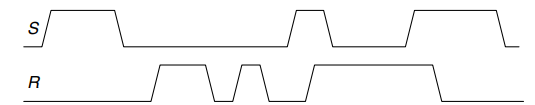
\includegraphics[width=0.6\textwidth]{03-01-input-waveform}
		\caption{Exercise 3-1: SR-Latch Input waveform}
		\label{03-01-input-waveform}
	\end{figure}
\end{ex}

\begin{sol}
	The output $Q$ is given in Figure~\ref{03-01-sr-latch-output}.
	\begin{figure}[h]
		\centering
		\includegraphics[width=0.6\textwidth]{03-01-sr-latch-output}
		\caption{Exercise 3-1: Output $Q$ for SR Latch from waveform}
		\label{03-01-sr-latch-output}
	\end{figure}
\end{sol}

\begin{ex}{3-2}
	Given the input waveforms shown in Figure~\ref{03-02-input-waveform}, sketch the output, $Q$, of an SR latch.
	\begin{figure}[h]
		\centering
		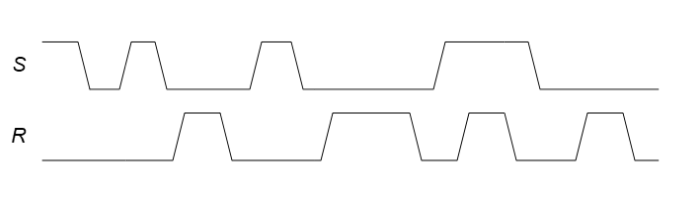
\includegraphics[width=0.6\textwidth]{03-02-input-waveform}
		\caption{Exercise 3-2: SR-Latch Input waveform}
		\label{03-02-input-waveform}
	\end{figure}
\end{ex}

\begin{sol}
	The output $Q$ is given in Figure~\ref{03-02-sr-latch-output}.
	\begin{figure}[h]
		\centering
		\includegraphics[width=0.6\textwidth]{03-02-sr-latch-output}
		\caption{Exercise 3-2: Output $Q$ for SR Latch from waveform}
		\label{03-02-sr-latch-output}
	\end{figure}
\end{sol}

\begin{ex}{3-3}
	Given the input waveforms shown in Figure~\ref{03-03-input-waveform}, sketch the output, $Q$, of a D latch.
	\begin{figure}[h]
		\centering
		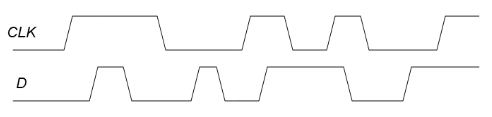
\includegraphics[width=0.6\textwidth]{03-03-input-waveform}
		\caption{Exercise 3-3: D-Latch Input waveform}
		\label{03-03-input-waveform}
	\end{figure}
\end{ex}

\begin{sol}
	The output $Q$ is given in Figure~\ref{03-03-D-latch-output}.
	\begin{figure}[h]
		\centering
		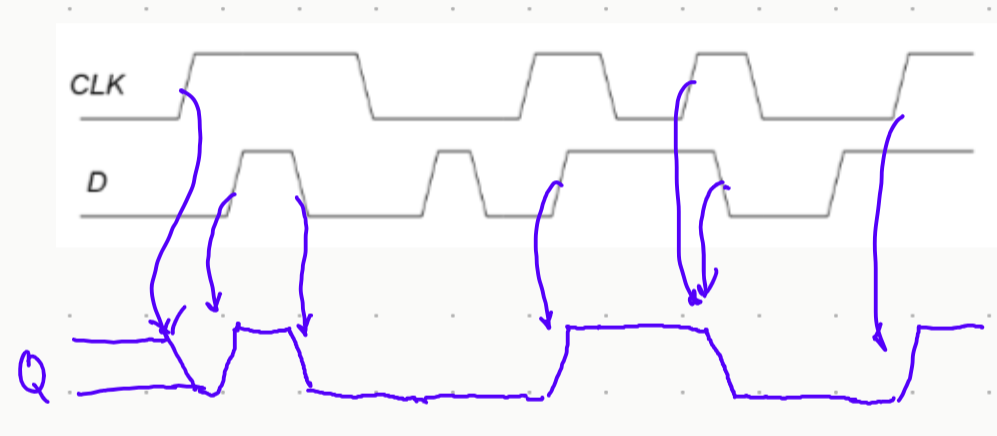
\includegraphics[width=0.6\textwidth]{03-03-D-latch-output}
		\caption{Exercise 3-3: Output $Q$ for D Latch from waveform}
		\label{03-03-D-latch-output}
	\end{figure}
\end{sol}

\begin{ex}{3-4}
	Given the input waveforms shown in Figure~\ref{03-04-input-waveform}, sketch the output, $Q$, of a D latch.
	\begin{figure}[h]
		\centering
		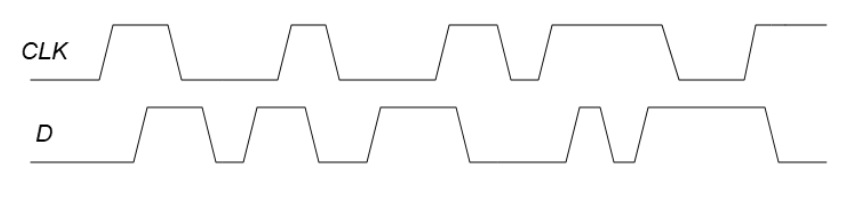
\includegraphics[width=0.6\textwidth]{03-04-input-waveform}
		\caption{Exercise 3-4: D-Latch Input waveform}
		\label{03-04-input-waveform}
	\end{figure}
\end{ex}

\begin{sol}
	The output $Q$ is given in Figure~\ref{03-04-D-latch-output}.
	\begin{figure}[h]
		\centering
		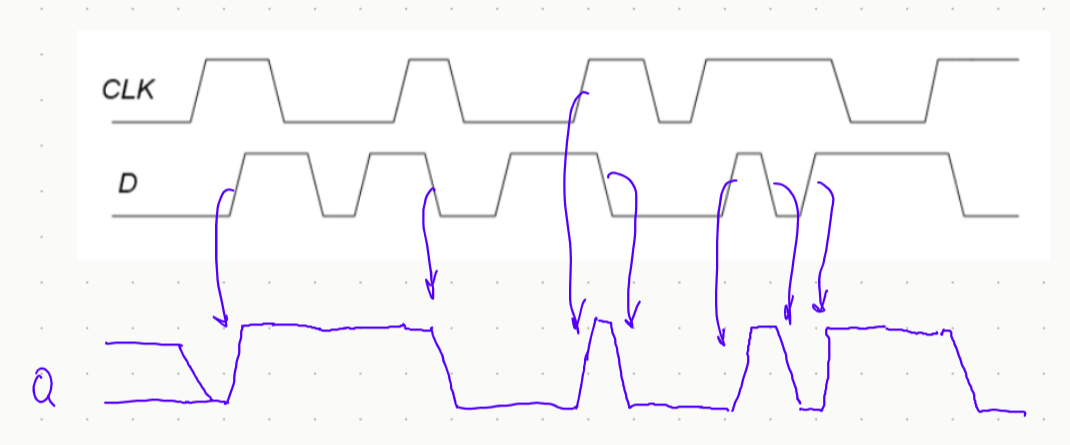
\includegraphics[width=0.6\textwidth]{03-04-D-latch-output}
		\caption{Exercise 3-4: Output $Q$ for D Latch from waveform}
		\label{03-04-D-latch-output}
	\end{figure}
\end{sol}

\begin{ex}{3.5}
	Given the input waveforms in Figure~\ref{03-03-input-waveform}, sketch the output, $Q$, of a flip-flop.
\end{ex}

\begin{sol}
	The output $Q$ is given in Figure~\ref{03-05-D-flip-flop-output}.
	\begin{figure}[h]
		\centering
		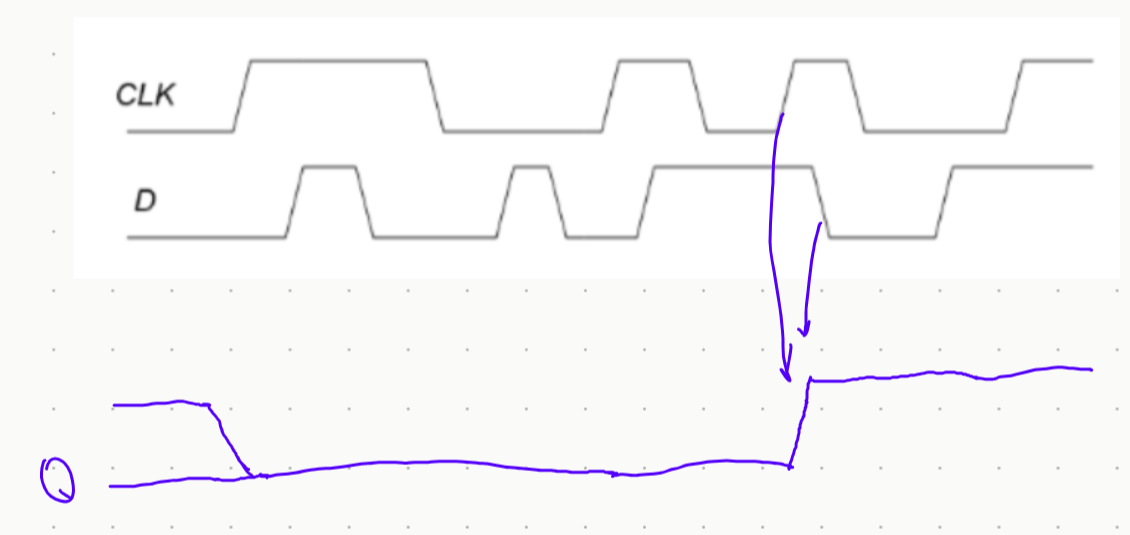
\includegraphics[width=0.6\textwidth]{03-05-D-flip-flop-output}
		\caption{Exercise 3-5: Output $Q$ for D Flip-Flop from waveform}
		\label{03-05-D-flip-flop-output}
	\end{figure}
\end{sol}

\begin{ex}{3.6}
	Given the input waveforms in Figure~\ref{03-04-input-waveform}, sketch the output, $Q$, of a flip-flop.
\end{ex}

\begin{sol}
	The output $Q$ is given in Figure~\ref{03-06-D-flip-flop-output}.
	\begin{figure}[h]
		\centering
		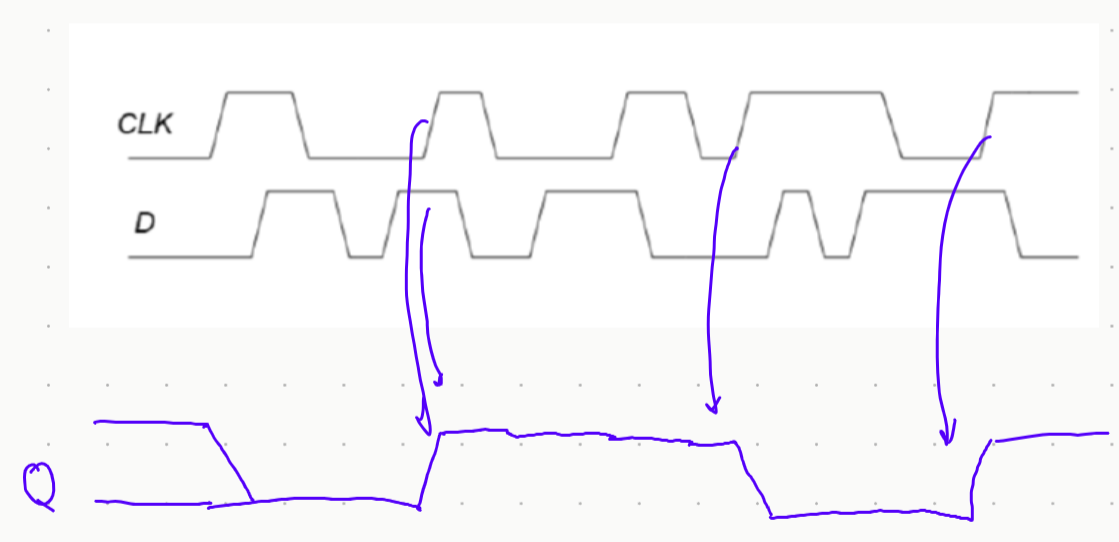
\includegraphics[width=0.6\textwidth]{03-06-D-flip-flop-output}
		\caption{Exercise 3-6: Output $Q$ for D Flip-Flop from waveform}
		\label{03-06-D-flip-flop-output}
	\end{figure}
\end{sol}

\begin{ex}{3.7}
	Is the circuit in Figure~\ref{03-07-nand-latch} combinational or sequential logic?
	Explain in a simple fashion what the relationship is between the
	inputs and outputs. What would you call this circuit?
	\begin{figure}[h]
		\centering
		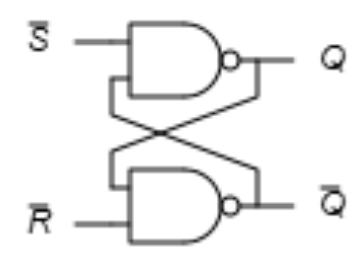
\includegraphics[width=0.2\textwidth]{03-07-nand-latch}
		\caption{Exercise 3-7: Mystery Circuit}
		\label{03-07-nand-latch}
	\end{figure}
\end{ex}

\begin{sol}
	It is not combinational because it has a cyclic path. It's possible that it's sequential. To understand what it does, we first examind all cases:
	\begin{itemize}
		\item Case 1: $\bar{R}=1$ and $\bar{S}=0$. The upper NAND gate sees a
		0, so it outputs 1 (regardless of the value of $Q$). The $1$ becomes an output for the second NAND gate, and since $\bar{R}=1$ also, the lower
		NAND gate outputs 0 for $\bar{Q}$.
		\item Case 2: $\bar{R}=0$ and $\bar{S}=1$. The upper NAND gate sees a 1,
		but without the value of $\bar{Q}$, we can't determine the output $Q$.
		Since the bottom NAND receives a 0 from $\bar{0}$, it outputs $1$
		for $\bar{Q}$. Revisiting the top NAND, now both inputs are $1$, making
		the output $0$ for $Q$.
		\item Case 3: $\bar{R}=0$ and $\bar{S}=0$. Since
		$\bar{S}=0$, the upper NAND outputs 1 for $Q$. Similarly, the lower NAND also outputs $1$ for $\bar{Q}$.
		\item Case 4: $\bar{R}=1$ and $\bar{S}=1$. If $Q$ has a known prior
		value $Q_{prev}$ before entering Case 4, $Q$ will remember this value,
		and $\bar{Q}_{prev}$ will be its complement, so this circuit has memory.
		See page 110 of the book.
		In this case, knowing the values $\bar{S}=1$ and $\bar{R}=1$ is not enough; we need to know $Q$. Suppose, as a subcase, that $Q=0$. Because $Q=0$, the bottom NAND gate outputs 1 for $\bar{Q}$. Now both inputs to the top NAND gate are 1, causing an output of $0$ for $Q$, as we assumed. If instead we assume that $Q=1$, then both inputs to the bottom NAND gate are 1, making the output 0 for $\bar{Q}$. Now since at least one input is $0$ for the top NAND gate, we get an output of 1 for $Q$, as we assumed initially. As described in page 109 through 110 of the book, this circuit has memory.
	\end{itemize}
	The truth table is summarized below:
	\begin{center}
		\begin{tabular}{cc|cc}
			$\bar{S}$ & $\bar{R}$ & $Q_{prev}$ & $\bar{Q}_{prev}$\\
			\hline
			0 & 0 & 1 & 1\\
			0 & 1 & 1 & 0\\
			1 & 0 & 0 & 1\\
			1 & 1 & $Q_{prev}$ & $\bar{Q}_{prev}$
		\end{tabular}
	\end{center}
	This is an SR-latch. It is a sequential circuit.
\end{sol}

\begin{ex}{3.8}
	Is the circuit in Figure~\ref{03-08-circuit} combinational logic or sequential logic? Explain in a simple
	fashion what the relationship is between the inputs and outputs. What would you call this
	circuit?
	\begin{figure}[h]
		\centering
		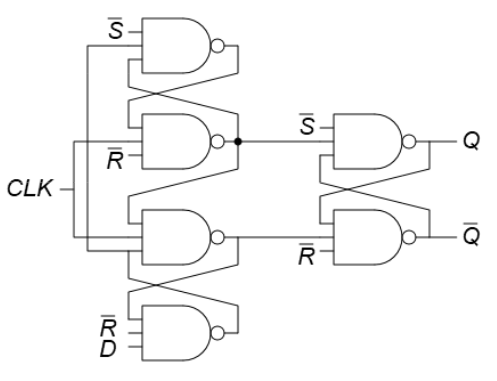
\includegraphics[width=0.6\textwidth]{03-08-circuit}
		\caption{Exercise 3-8: Mystery Circuit}
		\label{03-08-circuit}
	\end{figure}
\end{ex}

\begin{sol}
	The circuit implements sequential logic. It is controlled by a clock input CLK, and inputs depend on previous outputs. The table below shows the table of values:
	\begin{center}
		\begin{tabular}{cccc|cc}
			$CLK$ & $D$ & $\bar{S}$ & $\bar{R}$ & $Q$ & $\bar{Q}$\\
			\hline
			0 & 0 & 0 & 0 & 1 & 1\\
			0 & 0 & 0 & 1 & 1 & 0\\
			0 & 0 & 1 & 0 & 0 & 1\\
			0 & 0 & 1 & 1 & $Q_{prev}$ & $\bar{Q}_{prev}$\\
			0 & 1 & 0 & 0 & 1 & 1\\
			0 & 1 & 0 & 1 & 1 & 0\\
			0 & 1 & 1 & 0 & 0 & 1\\
			0 & 1 & 1 & 1 & $Q_{prev}$ & $\bar{Q}_{prev}$\\
			1 & 0 & 0 & 0 & 1 & 1\\
			1 & 0 & 0 & 1 & 1 & 0\\
			1 & 0 & 1 & 0 & 0 & 1\\
			1 & 0 & 1 & 1 & $Q_{prev}$ & $\bar{Q}_{prev}$ \\
			1 & 1 & 0 & 0 & 1 & 1\\
			1 & 1 & 0 & 1 & 1 & 0\\
			1 & 1 & 1 & 0 & 0 & 1\\
			1 & 1 & 1 & 1 & $Q_{prev}$ & $\bar{Q}_{prev}$\\
		\end{tabular}
	\end{center}
	Note that this is equivalent to the table in Exercise 3.7. Therefore, this must be an SR-latch.
\end{sol}

\begin{ex}{3.9}
	The \emph{toggle} ($T$) \emph{flip-flop} has one input, $CLK$, and one output, $Q$. On each rising edge of $CLK$,
	$Q$ toggles to the complement of its previous value. Draw a schematic for a $T$ flip-flop using a D flip-flop
	and an inverter.
\end{ex}

\begin{sol}
	See Figure~\ref{03-09-T-toggle-flip-flop}.
	\begin{figure}
		\centering
		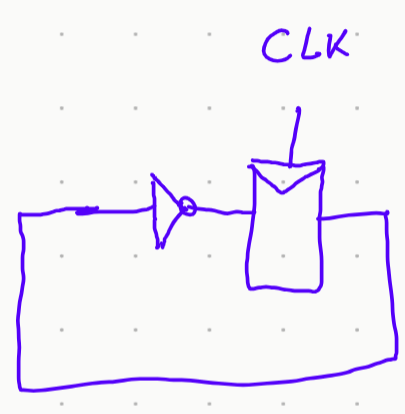
\includegraphics[width=0.3\textwidth]{03-09-T-toggle-flip-flop}
		\caption{Exercise 03-09: T (toggle) flip-flop}
		\label{03-09-T-toggle-flip-flop}
	\end{figure}
\end{sol}

\begin{ex}{3.10}
	A \emph{JK flip-flop} receives a clock and two inputs, \emph{J} and \emph{K}. On the rising edge of
	the clock, it updates the output, $Q$. If \emph{J} and \emph{K} are both 0, $Q$ retains its old value.
	If only $J$ is $1$, $Q$ becomes 1. If only $K$ is 1, $Q$ becomes 0. If both $J$ and $K$ are 1,
	$Q$ becomes the opposite of its present state.
	\begin{enumerate}[label=(\alph*)]
		\item Construct a JK flip-flop, using a D flip-flop and some combinational logic.
		\item Construct a D flip-flop, using a JK flip-flop and some combinational logic.
		\item Construct a T flip-flop (see Exercise 3.9), using a JK flip-flop.
	\end{enumerate}
\end{ex}

\begin{sol}\
	
	\begin{enumerate}[label=(\alph*)]
		\item The corresponding boolean equation is $Q=\bar{D}J+D\bar{K}$. When $CLK=0$, the logic from the flip-flop maintains the output unchanged. For $CLK=1$, we can create a boolean table based on the specification. The
		key is noting that the phrases "$Q$ retains its old value" or $Q$ becomes the opposite of its present state" can be explored by allowing it to be 0 or 1. Moreover, note that the output $Q$ is fed back as the input $D$. See the table below:
		\begin{center}
			\begin{tabular}{ccc|c}
				$D$ & $J$ & $K$ & $Q$\\
				\hline
				$0$ & $0$ & $0$ & $D=0$\\
				$0$ & $0$ & $1$ & $0$ \\
				$0$ & $1$ & $0$ & $1$\\
				$0$ & $1$ & $1$ & $\bar{D}=1$\\
				$1$ & $0$ & $0$ & $D=1$\\
				$1$ & $0$ & $1$ & $0$ \\
				$1$ & $1$ & $0$ & $1$\\
				$1$ & $1$ & $1$ & $\bar{D}=0$\\
			\end{tabular}
		\end{center}
		The corresponding Boolean equation is $Q=\bar{D}J+D\bar{K}$. See Figure~\ref{03-10a-jk-flip-flop}
		\begin{figure}
			\centering
			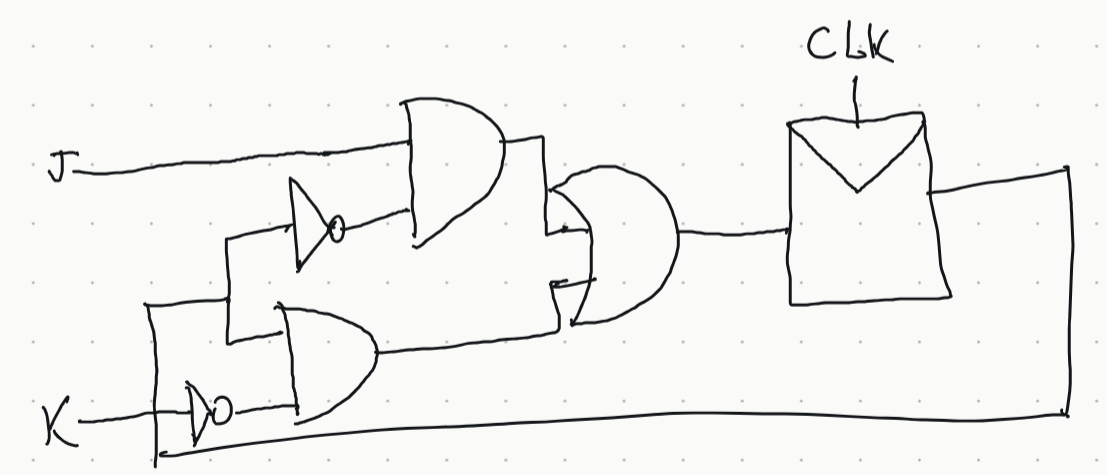
\includegraphics[width=0.6\textwidth]{03-10a-JK-flip-flop}
			\caption{Exercise 3.10: JK flip-flop built from D flip-flop and combinational logic}
			\label{03-10a-jk-flip-flop}
		\end{figure}
		\item To leverage the JK flip-flop, we feed its output back as its $K$ input, and $D$ as its $J$ input. See the table below, corresponding to what happens on the rising edge of the clock $(CLK=1)$.
		\begin{center}
			\begin{tabular}{cc|c}
				$D$ & $Q_{prev}$ & $Q$\\
				\hline
				0 & 0 & 0\\
				0 & 1 & 0\\
				1 & 0 & 1\\
				1 & 1 & 1\\
			\end{tabular}
		\end{center}
		Above, $D$ and $Q_{prev}$ are the inputs $J$ and $K$, respectively, to the JK flip-flop.
		\begin{figure}
			\centering
			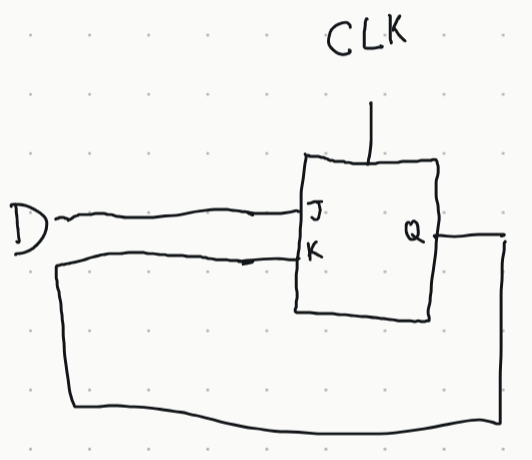
\includegraphics[width=0.5\textwidth]{03-10b-D-flip-flop}
			\caption{Exercise 3.11: D flip-flop built from JK flip-flop and combinational logic}
			\label{03-10b-D-flip-flop}
		\end{figure}
		\item See Figure~\ref{03-10c-T-flip-flop}
		\begin{figure}
			\centering
			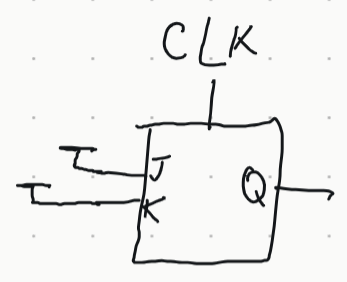
\includegraphics[width=0.5\textwidth]{03-10c-T-flip-flop}
			\caption{Exercise 3.11: T flip-flop built from JK flip-flop and combinational logic}
			\label{03-10c-T-flip-flop}
		\end{figure}
	\end{enumerate}
\end{sol}

\begin{ex}{3.12}
	Design an asynchronously resettable $D$ latch, using logic gates.
\end{ex}

\begin{sol}
	Asynchronously resettable means that when the reset input is false, it immediately outputs 0, rather
	than waiting for rising edge of the clock. In other words, when $Reset=1$, the output $Q$ becomes 0 regardless of $CLK$ and $D$. See Figure~\ref{03-12-async-resettable-D-latch}.
	\begin{figure}
		\centering
		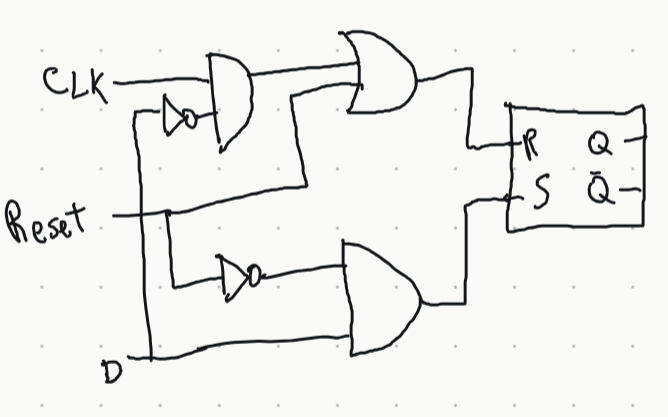
\includegraphics[width=0.5\textwidth]{03-12-async-resettable-D-latch}
		\caption{Exercise 3-12: Asynchronously resettable $D$-latch.}
		\label{03-12-async-resettable-D-latch}
	\end{figure}
\end{sol}

\begin{ex}{3.13}
	Design an asynchronously resettable $D$ flip-flop, using logic gates.
\end{ex}

\begin{sol}
	Asynchronously resettable means that when the reset input is 1, it immediately outputs 0, rather
	than waiting for rising edge of the clock. In other words, when $Reset=1$, the output $Q$ becomes 0 regardless of $CLK$ and $D$. See Figure~\ref{03-13-async-resettable-D-flip-flop}.
	\begin{figure}
		\centering
		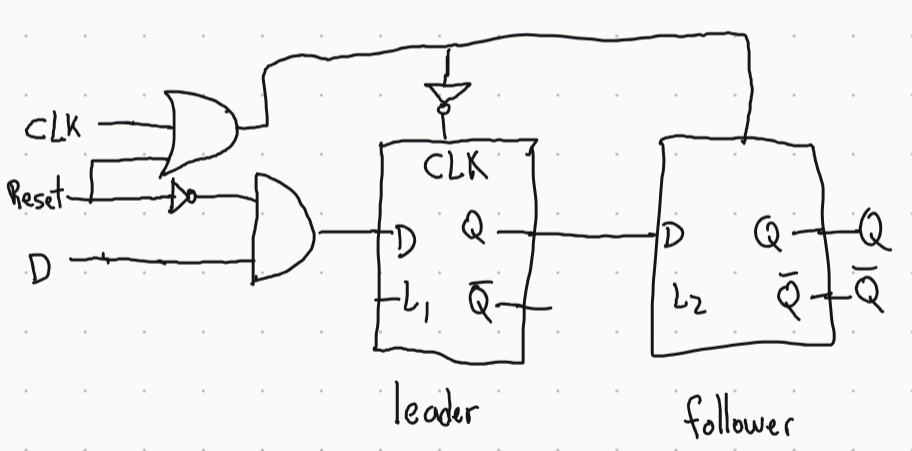
\includegraphics[width=0.7\textwidth]{03-13-async-resettable-D-flip-flop}
		\caption{Exercise 3-13: Asynchronously resettable $D$ flip-flop.}
		\label{03-13-async-resettable-D-flip-flop}
	\end{figure}
\end{sol}

\begin{ex}{3.14}
	Design an asynchronously settable $D$ latch, using logic gates.
\end{ex}

\begin{sol}
	Asynchronously settable means that when the set input is 1, it immediately outputs 1, rather
	than waiting for rising edge of the clock. In other words, when $Set=1$, the output $Q$ becomes 1 regardless of $CLK$ and $D$. See Figure~\ref{03-14-async-settable-D-latch}.
	\begin{figure}
		\centering
		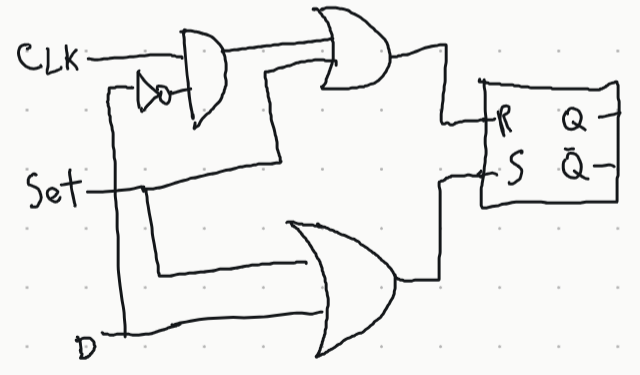
\includegraphics[width=0.6\textwidth]{03-14-async-settable-D-latch}
		\caption{Exercise 3-14: Asynchronously settable $D$ latch.}
		\label{03-14-async-settable-D-latch}
	\end{figure}
\end{sol}


\begin{ex}{3.15}
	Design an asynchronously settable $D$ flip-flop, using logic gates.
\end{ex}

\begin{sol}
	Asynchronously settable means that when the set input is 1, it immediately outputs 1, rather
	than waiting for rising edge of the clock. In other words, when $Set=1$, the output $Q$ becomes 1 regardless of $CLK$ and $D$. See Figure~\ref{03-15-async-settable-D-flip-flop}.
	\begin{figure}
		\centering
		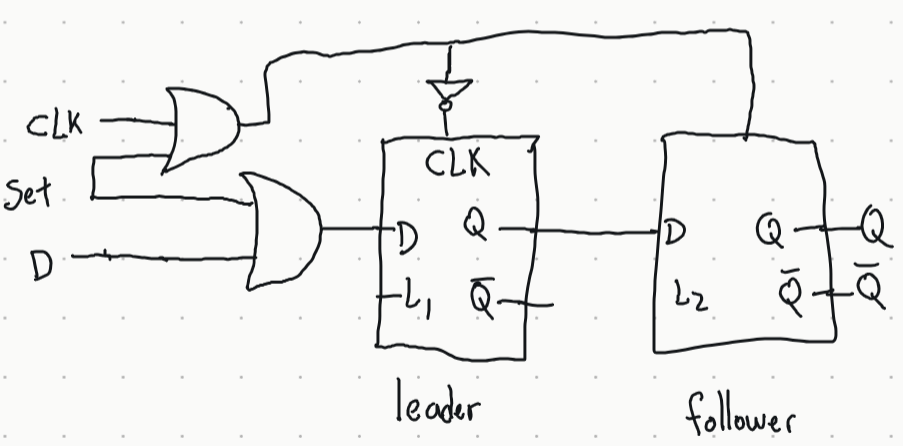
\includegraphics[width=0.6\textwidth]{03-15-async-settable-D-flip-flop}
		\caption{Exercise 3-15: Asynchronously settable $D$ flip-flop.}
		\label{03-15-async-settable-D-flip-flop}
	\end{figure}
\end{sol}

\begin{ex}{3.16}
	Suppose that a ring oscillator is built from $N$ inverters connected in a loop. Each inverter has a minimum
	delay of  $t_{cd}$, and a maximum delay of $t_{pd}$. If $N$ is odd, determine the range of frequencies
	at which the oscillator might operate.
\end{ex}

\begin{sol}
	Since $N$ is odd, there is an integer $k\in\mathbb{N}$ such that $N=2k-1$. Let the sequence of inverters, from
	left to right, be labeled $I_1,\ldots, I_{2k-1}$, and their corresponding input nodes be $M_{1},\ldots, M_{2_{k-1}}$. If $M_1$ is initially 0, then $M_2=0$, $M_3=1$, \ldots, $M_{2k-1}=0$, which feeds back into
	$I_1$ (and is $N_1$) with a value of 1. Hence, this circuit is unstable. \
	
	\
	
	If $M_1$ rises at time 0, then $M_2$ falls at time $t_{pd}$, $M_3$ rises at time $2t_{pd}$, and continuing on,
	$M_{2k+1}$ rises at time $2kt_{pd}$, which means $M_1$ will fall again at $(2k+1)t_{pd}$. This implies that
	$M_1$ rises again $(4k+2)t_{pd}$, or $2Nt_{pd}$. Therefore, each node oscillates with a period of $2Nt_{pd}$, or
	equivalently, with a frequency of $\frac{1}{2Nt_{pd}}$.
\end{sol}

\begin{ex}{3.17}
	Why must $N$ be odd in Exercise 3.16?
\end{ex}

\begin{sol}
	If $N$ is even, the circuit is stable. That is, if a node sees a bit value $D$, then it will always see
	that value. There is no oscillation, and hence frequency is undefined.
\end{sol}

\begin{ex}{3.18}
	Which of the circuits in Figure~\ref{03-18-circuits} are synchronous sequential circuits? Explain.
	\begin{figure}[h]
		\centering
		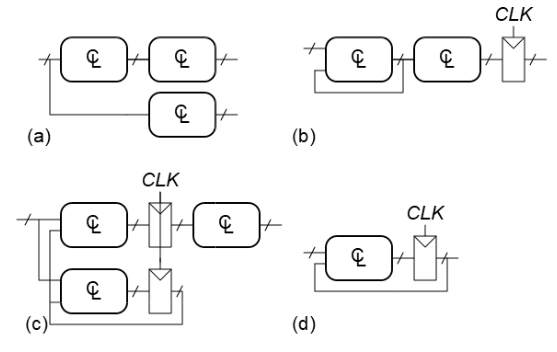
\includegraphics[width=0.7\textwidth]{03-18-circuits}
		\caption{Exercise 3-18: Circuits}
		\label{03-18-circuits}
	\end{figure}
\end{ex}

\begin{sol}
	\
	A synchronous sequential circuit has a clock input, whose rising edges indicate a sequence of times at which
	state transitions occur. The rules of synchronous sequential composition say that a circuit is a
	synchronous sequential circuit of interconnected circuit elements, such that
	\begin{enumerate}
		\item Every circuit element is either a register, or a combinational circuit.
		\item At least one circuit element is a register.
		\item All registers receive the same clock signal.
		\item Every cyclic path contains at least one register.
	\end{enumerate}
	\begin{enumerate}[label=(\alph*)]
		\item This is a combinational circuit.
		\item This is not a combinational circuit because of the cycle at the node that follows the leftmost combinational element. It is not a synchronous sequential circuit because the cyclic path does not contain the one register in the circuit.
		\item There are two registers, both receiving the same clock signal, and every circuit element is combinational or a register. There is a cycle path starting at the node that is the output of the lower combinational element, and it includes a register, so this is a synchronous sequential circuit.
		\item There is one register and one combinational element. There is a cyclic path containing the node that is the output of the combinational output, and since it includes the register, it follows that this is a
		synchronous sequential circuit.
	\end{enumerate}
\end{sol}

\begin{ex}{3.19}
	You are designing an elevator controller for a building with 25 floors. The controller has two inputs:
	UP and DOWN. It produces an output indicating the floor the elevator is on. There is no floor 13. What is
	the minimum number of bits of state in the controller?
\end{ex}

\begin{sol}
	The state represents the current floor that the elevator is on. If using binary encoding, then 23 floors (since 13 is not included) needs $\ceil{\log_2{23}}=5$ floors. If using one-hot encoding, it would be 23 bits of state.
\end{sol}

\begin{ex}{3.20}
	You are designing an FSM to keep track of the mood of four students working in the digital design lab.
	Each student's mood is either HAPPY (the circuit works), SAD (the circuit blew up), BUSY (working on the
	circuit), CLUELESS (confused about the circuit), or ASLEEP (face down on the circuit board). How many
	states does the FSM have? What is the minimum number of bits necessary to represent these states?
\end{ex}

\begin{sol}
	There are $5^4$ states because we are tracking the mood of all four students and each student can be in
	one of five moods, so we need $\ceil{\log_2(5^4)}$ bits, or at least 10 bits.
\end{sol}

\begin{ex}{3.21}
	How would you factor the FSM from Exercise 3.20 into multiple simpler machines? How many states does
	each simpler machine have? What is the minimum total number of bits necessary into this factored
	design?
\end{ex}

\begin{sol}
	A factored design could include 1 state machine for each student. Since a student can be in 5 moods, each
	student's state requires $\ceil{\log_2{5}}=3$ states. Hence, for 4 students, that's a total of 12 bits.
\end{sol}

\begin{ex}{3.22}
	Describe in words what the state machine in Figure~\ref{03-22-state-machine} does. Using binary state encodings, complete
	a state transition table and output table for the FSM. Write Boolean equations for the next state and output
	and sketch a schematic of the FSM.
	\begin{figure}
		\centering
		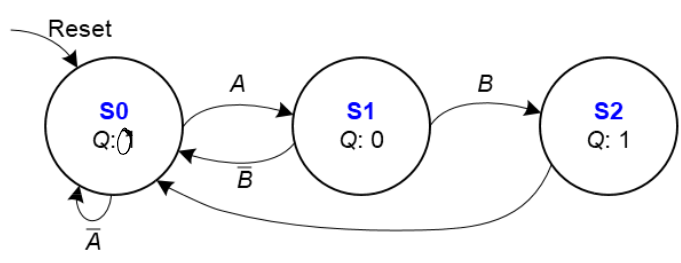
\includegraphics[width=0.5\textwidth]{03-22-state-machine}
		\caption{Exercise 3-22: State machine.}
		\label{03-22-state-machine}
	\end{figure}
\end{ex}
\begin{sol}
	The machine starts in state $S0$ and remains there until $A=1$.  At that point, it transitions to $S1$,
	transitioning to S2 if $B=1$ or returning to $S0$ if $B=0$. Once at $S2$, it unconditionally returns to S0.
	The state transition table is below. The output is $1$ when it reaches $S_2$, and its 0 otherwise.
	\begin{center}
		\begin{tabular}{c|cc|c}
			$S$ & $A$ & $B$ & $S'$\\
			\hline
			$S0$ & $0$ & $X$ & $S0$\\
			$S0$ & $1$ & $X$ & $S1$\\
			$S1$ & $X$ & $0$ & $S0$\\
			$S1$ & $X$ & $1$ & $S2$\\
			$S2$ & $X$ & $X$ & $S0$\\
		\end{tabular}
	\end{center}
	Below are the state encoding, state transition, and output tables:
	\begin{center}
		\begin{tabular}{c|c}
			State & Encoding\\
			\hline
			$S0$ & $00$\\
			$S1$ & $01$\\
			$S2$ & $10$\\
		\end{tabular}
		\quad
		\begin{tabular}{cc|cc|cc}
			$S_1$ & $S_0$ & $A$ & $B$ & $S_1'$ & $S_0'$\\
			\hline
			$0$ & $0$ & $0$ & $X$ & $0$ & $0$\\
			$0$ & $0$ & $1$ & $X$ & $0$ & $1$\\
			$0$ & $1$ & $X$ & $0$ & $0$ & $0$\\
			$0$ & $1$ & $X$ & $1$ & $1$ & $0$\\
			$1$ & $0$ & $X$ & $X$ & $0$ & $0$\\
		\end{tabular}
		\quad 
		\begin{tabular}{cc|c}
			$S_1$ & $S_0$ & $Q$\\
			\hline
			$0$ & $0$ & $0$\\
			$0$ & $1$ & $0$\\
			$1$ & $0$ & $1$\\
		\end{tabular}
	\end{center}
	After creating K-Maps (with don't-cares for $S_1S_0=11$), the
	simplified equations become:
	\begin{align*}
		Q&=S_1\\
		S_0'&=\bar{S_0}\bar{S_1}A\\
		S_1'&=BS_0
	\end{align*}
	The corresponding circuit is in Figure~\ref{03-22-circuit}.
	\begin{figure}
		\centering
		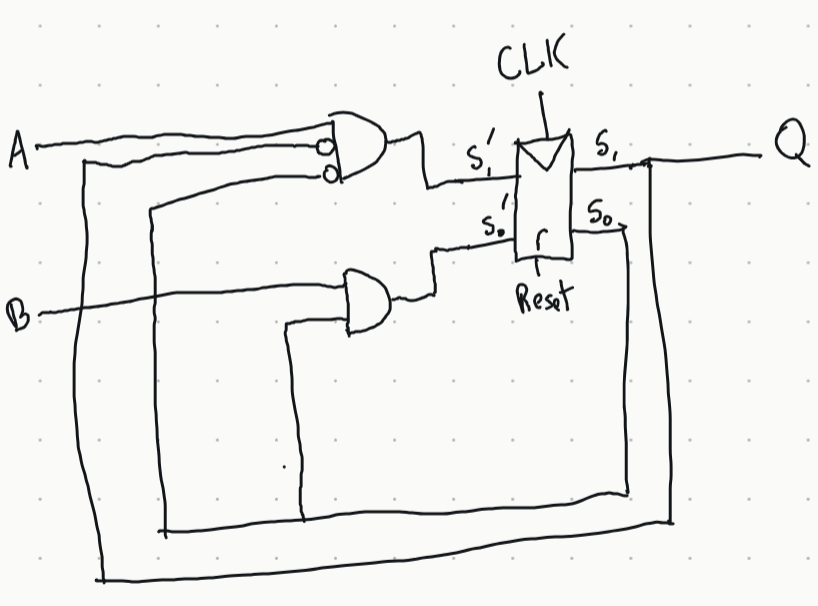
\includegraphics[width=0.5\textwidth]{03-22-circuit-schematic}
		\caption{Exercise 3-22: Circuit from State Machine in
			Figure~\ref{03-22-state-machine}}
		\label{03-22-circuit}
	\end{figure}
\end{sol}

\begin{ex}{3.23}
	Describe in words what the state machine in Figure~\ref{03-23-state-machine} does. Use binary state encodings,
	complete a state transition table and output table for the FSM.
	Write Boolean equations for the next state and output, and sketch
	a schematic of the FSM.
	\begin{figure}
		\centering
		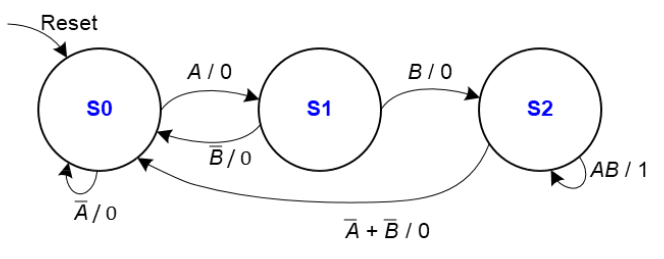
\includegraphics[width=0.5\textwidth]{03-23-state-machine}
		\caption{Exercise 3-23: State transition diagram}
		\label{03-23-state-machine}
	\end{figure}
\end{ex}

\begin{sol}
	This one is a Mealy state machine, since the output depends
	on both the state and inputs. The state machine outputs 0
	unless $A=B=1$ while it is in state $S2$.
	It starts in state $S0$, and remains there while $A=0$.
	When $A=1$, it transitions to $S2$. From here, if $B=0$,
	it returns to state 0, and otherwise it transitions to
	$S2$. It then remains at state $S2$ while $A=0$ or $B=0$,
	in which case it returns to state $S0$. Below is the state
	encoding table using binary encoding:
	\begin{center}
		\begin{tabular}{c|c}
			State & Encoding\\
			\hline
			$S0$ & $00$\\
			$S1$ & $01$\\
			$S2$ & $10$\\
		\end{tabular}
	\end{center}
	The state transition and output tables are given below:
	\begin{center}
		\begin{tabular}{cc|cc|cc}
			$S_1$ & $S_0$ & $A$ & $B$ & $S_1'$ & $S_0'$\\
			\hline
			$0$ & $0$ & $0$ & $X$ & $0$ & $0$\\
			$0$ & $0$ & $1$ & $X$ & $0$ & $1$\\
			$0$ & $1$ & $X$ & $0$ & $0$ & $0$\\
			$0$ & $1$ & $X$ & $1$ & $1$ & $0$\\
			$1$ & $0$ & $0$ & $0$ & $0$ & $0$\\
			$1$ & $0$ & $0$ & $1$ & $0$ & $0$\\
			$1$ & $0$ & $1$ & $0$ & $0$ & $0$\\
			$1$ & $0$ & $1$ & $1$ & $1$ & $0$
		\end{tabular}
		\quad
		\begin{tabular}{cc|cc|c}
			$S_1$ & $S_0$ & $A$ & $B$ & $Q$\\
			\hline
			$0$ & $0$ & $X$ & $X$ & $0$ \\
			$0$ & $1$ & $X$ & $X$ & $0$ \\
			$1$ & $0$ & $0$ & $0$ & $0$ \\
			$1$ & $0$ & $0$ & $1$ & $0$ \\
			$1$ & $0$ & $1$ & $0$ & $0$ \\
			$1$ & $0$ & $1$ & $1$ & $1$ \\
		\end{tabular}
	\end{center}
	The corresponding Boolean equations are:
	\begin{align*}
		S_1'&=S_0B+S_1AB\\
		S_0'&=\bar{S_1}\bar{S_0}A\\
		Q&=S_1AB
	\end{align*}
	Finally, the circuit is in Figure~\ref{03-23-circuit-schematic}.
	\begin{figure}
		\centering
		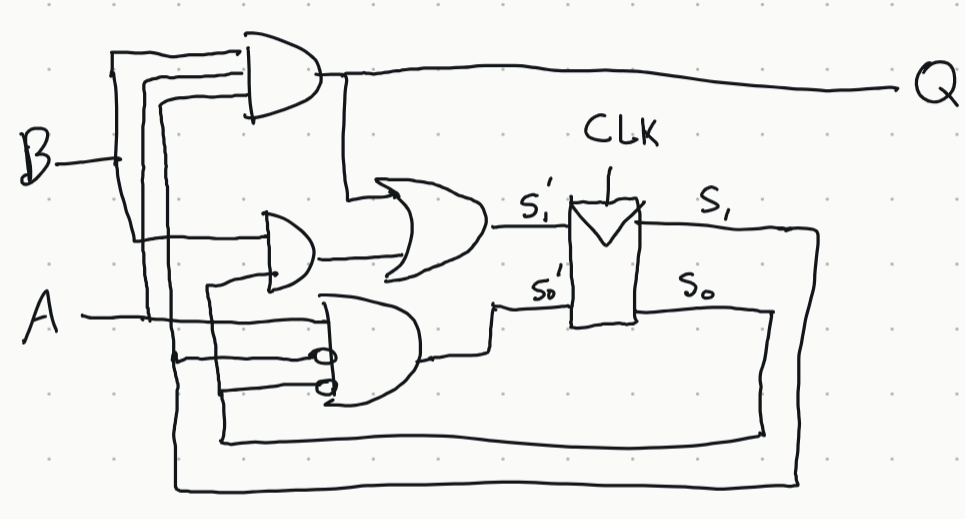
\includegraphics[width=0.6\textwidth]{03-23-circuit-schematic}
		\caption{Exercise 03-23: Circuit schematic for State Machine in Figure~\ref{03-23-state-machine}}
		\label{03-23-circuit-schematic}
	\end{figure}
\end{sol}

\begin{ex}{3.24}
	Accidents are still occurring at the intersection of Academic
	Avenue and Bravado Boulevard. The football team is rushing into the
	intersection the moment light $B$ turns green. They are colliding
	with sleep-deprived CS majors who stagger into the intersection
	just before light A turns red. Extend the traffic light controller
	from Section 3.4.1 so that both lights are red for 5 seconds before
	either light turns green again. Sketch your improved Moore machine
	state transition diagram, state encodings, state transition table,
	output table, next state and output equations, and your FSM
	schematic.
\end{ex}

\begin{sol}
	The states for yellow lights each wait 5 seconds before switching. We can make a similar state that follows each yellow light state. See Figure~\ref{03-24-state-machine}.
	\begin{figure}
		\centering
		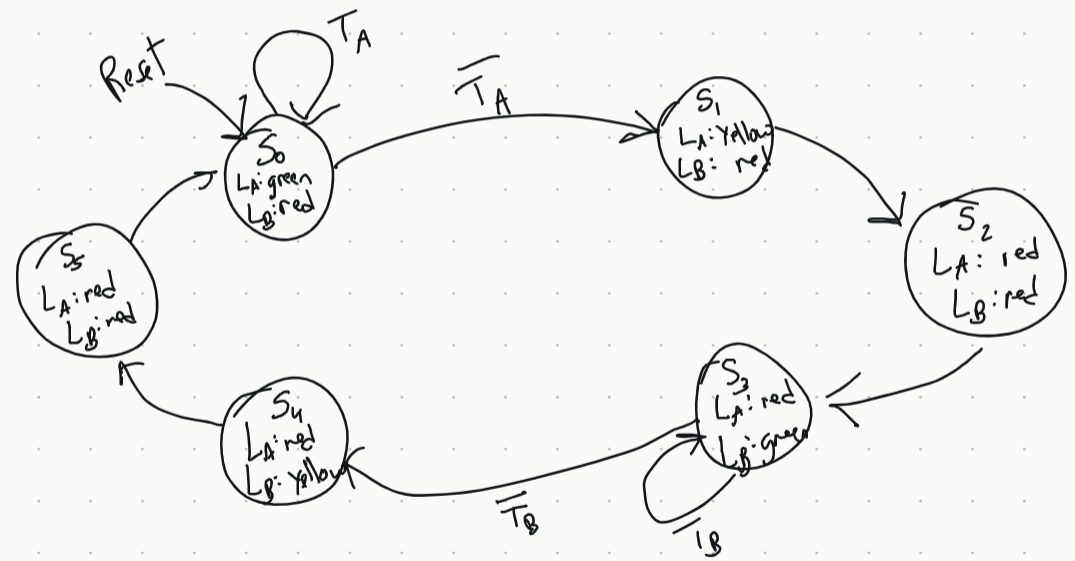
\includegraphics[width=0.7\textwidth]{03-24-state-machine}
		\caption{Exercise 3-24: State Machine with red light states}
		\label{03-24-state-machine}
	\end{figure}
	Now that two new states have been added, the states have been relabeled, and an extra bit is necessary. The output encoding is also present.
	\begin{center}
		\begin{tabular}{c|c}
			State & Encoding $S_{2:0}$ \\
			\hline
			$S0$ & $000$\\
			$S1$ & $001$\\
			$S2$ & $010$\\
			$S3$ & $011$\\
			$S4$ & $100$\\
			$S5$ & $101$\\
		\end{tabular}
		\quad
		\begin{tabular}{c|c}
			Output & Encoding $L_{1:0}$\\
			\hline
			green & $00$\\
			yellow & $01$\\
			red & $10$\\
		\end{tabular}
	\end{center}
	The state transition table and output table are below:
	\begin{center}
		\begin{tabular}{ccc|cc|ccc}
			$S_2$ & $S_1$ & $S_0$ & $T_A$ & $T_B$ & $S_{2}'$ & $S_{1}'$ & $S_0'$\\
			\hline
			$0$ & $0$ & $0$ & $0$ & $X$ & $0$ & $0$ & $1$\\
			$0$ & $0$ & $0$ & $1$ & $X$ & $0$ & $0$ & $0$\\
			$0$ & $0$ & $1$ & $X$ & $X$ & $0$ & $1$ & $0$\\
			$0$ & $1$ & $0$ & $X$ & $X$ & $0$ & $1$ & $1$\\
			$0$ & $1$ & $1$ & $X$ & $0$ & $1$ & $0$ & $0$\\
			$0$ & $1$ & $1$ & $X$ & $1$ & $0$ & $1$ & $1$\\
			$1$ & $0$ & $0$ & $X$ & $X$ & $1$ & $0$ & $1$\\
			$1$ & $0$ & $1$ & $X$ & $X$ & $0$ & $0$ & $0$\\
		\end{tabular}
		\quad
		\begin{tabular}{ccc|cccc}
			$S_2$ & $S_1$ & $S_0$ & $L_{A1}$ & $L_{A0}$ & $L_{B1}$ & $L_{B0}$\\
			\hline
			$0$ & $0$ & $0$ & $0$ & $0$ & $1$ & $0$\\
			$0$ & $0$ & $1$ & $0$ & $1$ & $1$ & $0$\\
			$0$ & $1$ & $0$ & $1$ & $0$ & $1$ & $0$\\
			$0$ & $1$ & $1$ & $1$ & $0$ & $0$ & $0$\\
			$1$ & $0$ & $0$ & $1$ & $0$ & $0$ & $1$\\
			$1$ & $0$ & $1$ & $1$ & $0$ & $1$ & $0$\\
		\end{tabular}
	\end{center}
	The output equations are:
	\begin{align*}
		L_{A1}&=\bar{S_2}S_1\bar{S_0}+\bar{S_2}S_1S_0+S_2\bar{S_1}\bar{S_0}+S_2\bar{S_1}S_0\\
		&=\bar{S_2}S_1+S_2\bar{S_1}\\
		&=S_2\oplus S_1\\
		L_{A0}&=\bar{S_2}\bar{S_1}S_0\\
		L_{B1}&=\bar{S_2}\bar{S_1}\bar{S_0}+\bar{S_2}\bar{S_1}S_0
		+\bar{S_2}S_1\bar{S_0}+S_2\bar{S_1}S_0\\
		&=\bar{S_2}\bar{S_0}+\bar{S_1}S_0\\
		L_{B0}&=S_2\bar{S_1}\bar{S_0}
	\end{align*}
	The next state equations are:
	\begin{align*}
		S_{2}'&=\bar{S_2}S_1S_0\bar{T_B}+S_2\bar{S_1}\bar{S_0}T_B\\
		&=\bar{S_2}S_1S_0+S_2\bar{S_1}\bar{S_0}\\
		S_{1}'&=\bar{S_2}\bar{S_1}S_0
		+\bar{S_2}S_1\bar{S_0}
		+\bar{S_2}S_1S_0T_B\\
		S_{0}'&=\bar{S_2}\bar{S_1}\bar{S_0}\bar{T_A}+\bar{S_2}S_1\bar{S_0}
		+\bar{S_2}S_1S_0T_B+S_2\bar{S_1}\bar{S_0}		
	\end{align*}
	I'll skip creating the circuit.
\end{sol}

\begin{ex}{3.25}
	Alyssa P Hacker's snail from Section 3.4.3 has a daughter with a Mealy machine FSM brain.
	The daughter snail smiles whenever she slides over the pattern $1101$ or the pattern $1110$.
	Sketch the state transition diagram for the happy snail using as a few states as possible.
	Choose state encodings and write a combined state transition and output table, using your
	encodings. Write the new state and output equations and sketch your FSM schematic.
\end{ex}

\begin{sol}
	Figure~\ref{03-25-mealy-state-machine} shows the Mealy state machine diagram.
	\begin{figure}
		\centering
		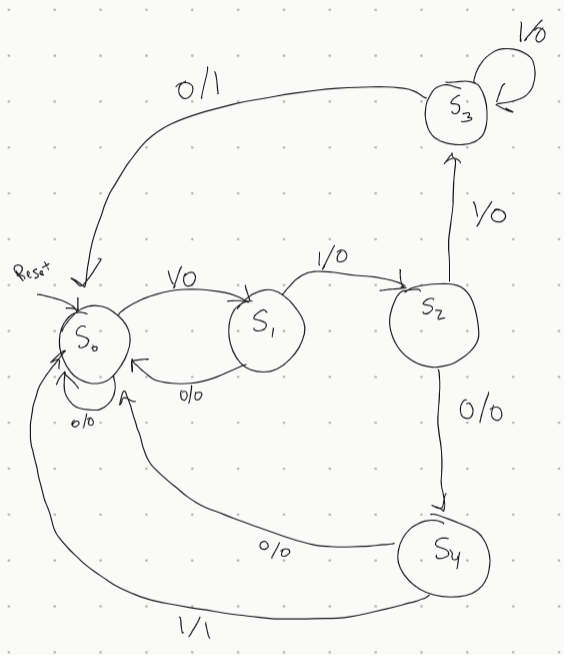
\includegraphics[width=0.5\textwidth]{03-25-mealy-state-machine}
		\caption{Exercise 3-25: Mealy State Machine}
		\label{03-25-mealy-state-machine}
	\end{figure}
	We begin at state $S0$, and all state transitions result in an output of $0$,
	except for state transitions to $S0$ from $S3$ and $S4$ when the inputs are
	$0$ and $1$, respectively.
\end{sol}

\begin{ex}{3.26}
	You have been enlisted to design a soda machine dispenser for your department lounge.
	Sodas are partially subsidized by the student chapter of the IEEE, so they cost only
	25 cents. The machine accepts nickels, dimes, and quarters. When enough coins have been
	inserted, it dispenses the soda and returns any necessary change. Design an FSM
	controller for the soda machine. The FSM inputs are \emph{Nickel}, \emph{Dime}, and \emph{Quarter},
	indicating which coin was inserted. Assume that exactly one coin is inserted on each cycle.
	The outputs are \emph{Dispense}, \emph{ReturnNickel}, \emph{ReturnDime}, and \emph{ReturnTwoDimes}.
	When the FSM reaches 25 cents, it asserts \emph{Dispense} and the necessary \emph{Return}
	outputs required to deliver the appropriate change. Then, it should be ready to start
	accepting coins for another soda.
\end{ex}
\begin{sol}
	The Moore state machine is given in Figure~\ref{03-26-state-machine}.
	\begin{figure}
		\centering
		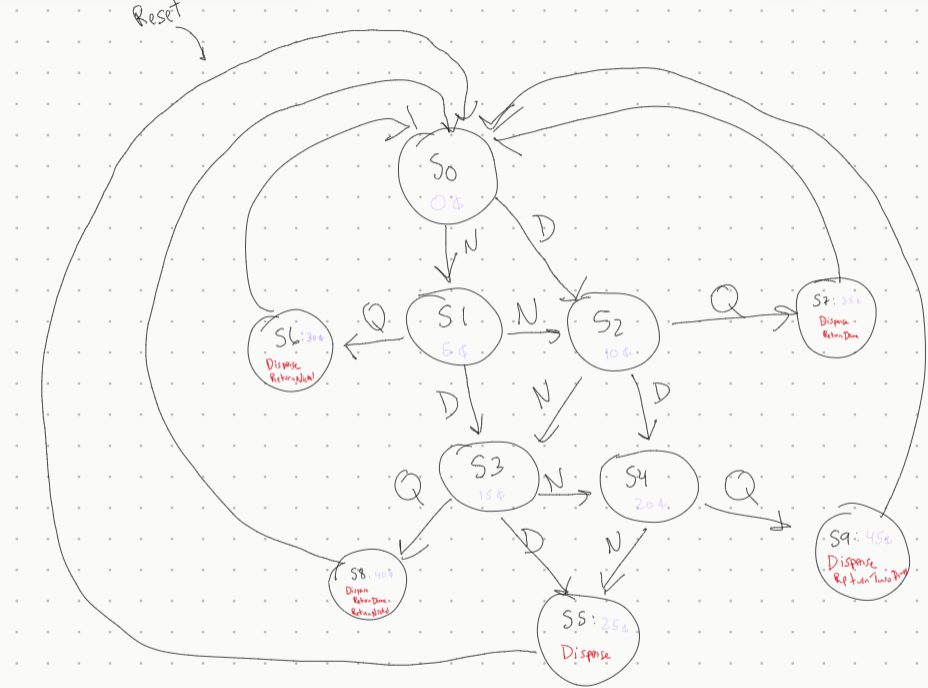
\includegraphics[width=0.8\textwidth]{03-26-state-machine}
		\caption{Exercise 03-26: Moore state machine}
		\label{03-26-state-machine}
	\end{figure}
	The state $S$ represents the current amount of money in the vending machine.
	The following tables show the mapping of state names, and input names.
	\begin{center}
		\begin{tabular}{c|c}
			State & Amount of Money\\
			\hline
			$S0$ & $0$ \textcent\\
			$S1$ & $5$ \textcent\\
			$S2$ & $10$ \textcent\\
			$S3$ & $15$ \textcent\\
			$S4$ & $20$ \textcent\\
			$S5$ & $25$ \textcent\\
			$S6$ & $30$ \textcent\\
			$S7$ & $35$ \textcent\\
			$S8$ & $40$ \textcent\\
			$S9$ & $45$ \textcent\\
		\end{tabular}
		\quad
		\begin{tabular}{cc}
			Input & Shorthand\\
			\hline
			\emph{Nickel} & $N$\\
			\emph{Dime} & $D$\\
			\emph{Quarter} & $Q$\\
		\end{tabular}
	\end{center}
	For states $S0$ through $S4$, all outputs are FALSE (and thus not asserted). The
	following table shows the outputs asserted:
	\begin{center}
		\begin{tabular}{cc}
			State & Outputs\\
			\hline
			$S5$ & \emph{Dispense}\\
			$S6$ & \emph{Dispense}, \emph{ReturnNickel}\\
			$S7$ & \emph{Dispense}, \emph{ReturnDime}\\
			$S8$ & \emph{Dispense}, \emph{ReturnDime}, \emph{ReturnNickel}\\
			$S9$ & \emph{Dispense}, \emph{ReturnTwoDimes}
		\end{tabular}
	\end{center}
\end{sol}

\begin{ex}{3.27}
	Gray codes have a useful property in that consecutive numbers differ in only a single
	position. The table below lists a 3-bit Gray code representing the numbers 0 to 7.
	
	\begin{center}
		\begin{tabular}{c|ccc}
			Number & \multicolumn{3}{c}{Gray code}\\
			\hline
			0 & 0 & 0 & 0\\
			1 & 0 & 0 & 1\\
			2 & 0 & 1 & 1\\
			3 & 0 & 1 & 0\\
			4 & 1 & 1 & 0\\
			5 & 1 & 1 & 1\\
			6 & 1 & 0 & 1\\
			7 & 1 & 0 & 0\\
		\end{tabular}
	\end{center}
	
	Design a 3-bit modulo 8 Gray code counter FSM with no inputs and three outputs.
	(A modulo $n$ counts from 0 to $N-1$, then repeats. For example, a watch uses a modulo
	60 counter for the minutes and seconds that counts from 0 to 59). When reset, the output should be $000$. On each clock edge, the output should advance to the next Gray code. After reaching
	$100$, it should repeat with $000$.
\end{ex}

\begin{sol}
	The state machine is in Figure~\ref{03-27-state-machine}.
	\begin{figure}
		\centering
		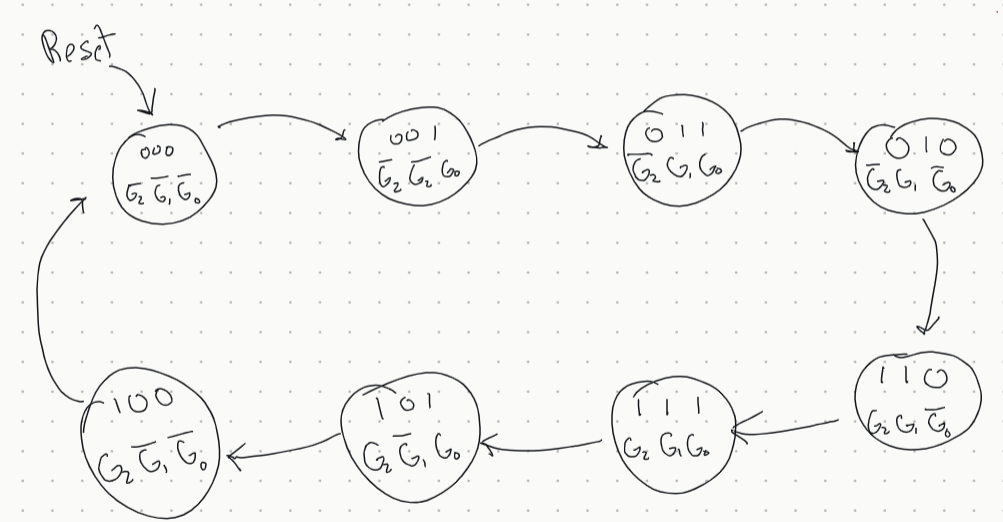
\includegraphics[width=0.8\textwidth]{03-27-state-machine}
		\caption{Exercise 03-27: State machine}
		\label{03-27-state-machine}
	\end{figure}
\end{sol}

\begin{ex}{3.28}
	Extend your modulo 8 Gray code counter from Exercise 3.27 to be an UP/DOWN counter
	by adding an \emph{UP} input. If \emph{UP = 1}, the counter advances to the next number.
	If $UP=0$, the counter retreats to the previous number.
\end{ex}

\begin{sol}
	The state machine is in Figure~\ref{03-28-state-machine}.
	\begin{figure}
		\centering
		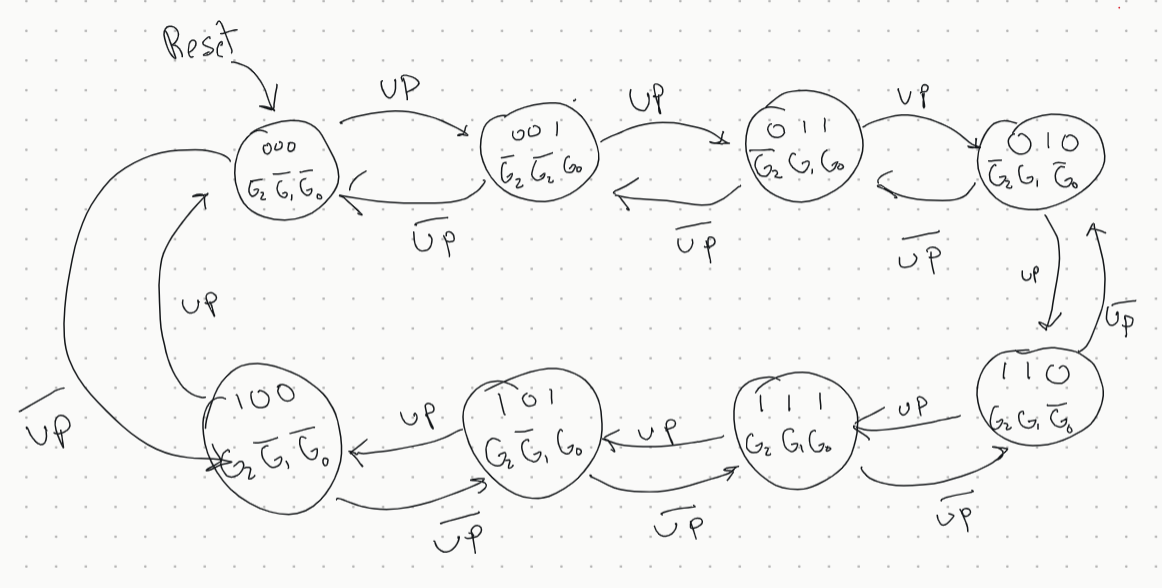
\includegraphics[width=0.8\textwidth]{03-28-state-machine}
		\caption{Exercise 03-28: State machine}
		\label{03-28-state-machine}
	\end{figure}
\end{sol}

\begin{ex}{3.29}
	Your company, Detect-o-rama, would like to design an FSM that takes two inputs,
	$A$ and $B$, and generate one output, $Z$. The output in cycle $n$, $Z_n$, is
	either the Boolean AND or OR of the corresponding input $A_n$ and the previous
	input $A_{n-1}$, depending on the other input, $B_n$:
	\begin{align*}
		Z_n&=A_nA_{n-1}\quad \text{if}\quad B_n=0\\
		Z_n&=A_n+A_{n-1}\quad \text{if}\quad B_n=1\\
	\end{align*}
	\begin{enumerate}[label=(\alph*)]
		\item Sketch the waveform for $Z$, given the inputs shown in Figure~\ref{03-29-input-waveform}.
		\item Is this FSM a Moore or a Mealy machine?
		\item Design the FSM. Show your state transition diagram, encoded state
		transition table, next state and output equations, and schematic.
	\end{enumerate}
	\begin{figure}
		\centering
		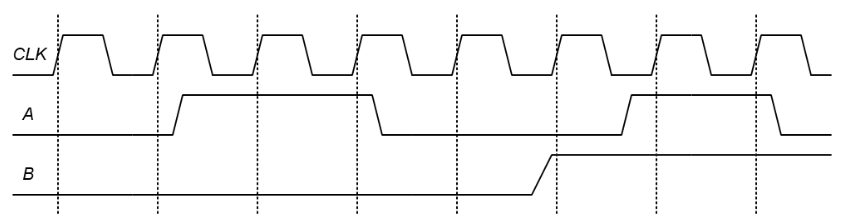
\includegraphics[width=0.8\textwidth]{03-29-input-waveform}
		\caption{FSM input waveforms for Exercise 3.29}
		\label{03-29-input-waveform}
	\end{figure}
\end{ex}

\begin{sol}
	\begin{enumerate}[label=(\alph*)]
		\item See Figure~\ref{03-29-output-waveform}.
		\begin{figure}
			\centering
			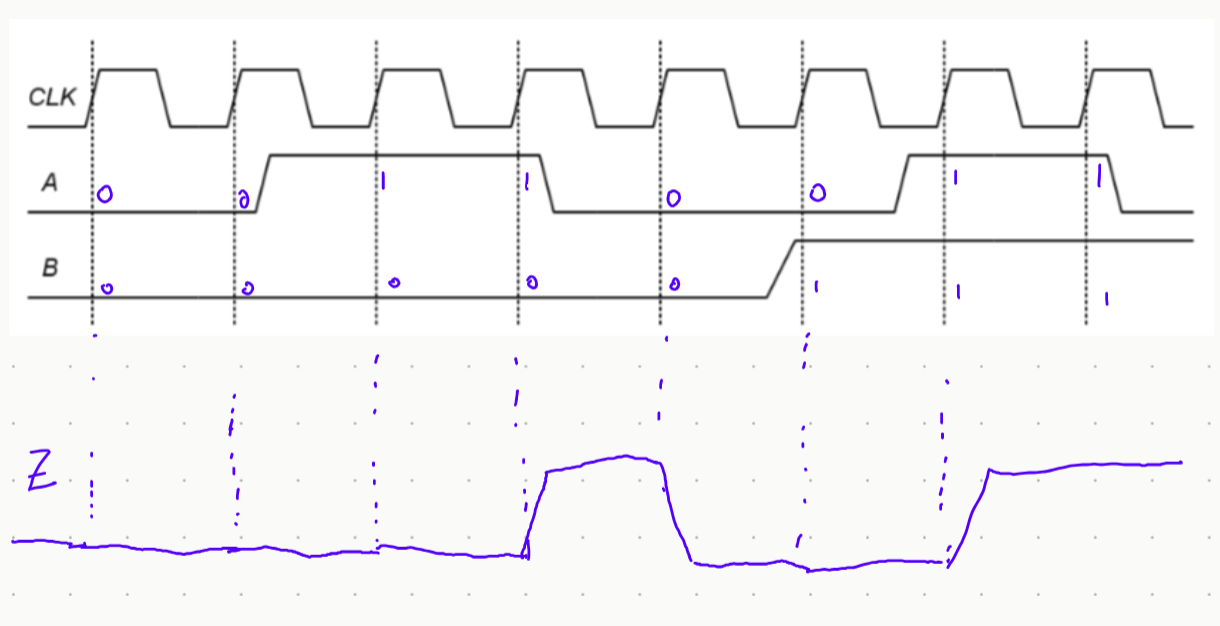
\includegraphics[width=0.6\textwidth]{03-29-output-waveform}
			\caption{Output waveform for Exercise 3.29 (a)}
			\label{03-29-output-waveform}
		\end{figure}
		\item A Moore state machine depends only on the current state of the machine.
		However, this FSM depends both on the current state, namely the value of $A_{n-1}$,
		and the inputs $A_n$ and $B_n$. Therefore, this is a Mealy state machine.
		\item See Figure~\ref{03-29-state-machine}. The state $S$ is the previous
		value of the input, $A_{n-1}$, and it can be represented by a single bit.
		State $S0$ corresponds to $A_{n-1}=0$, and state $S1$ corresponds to $A_{n-1}=1$.
		\begin{figure}
			\centering
			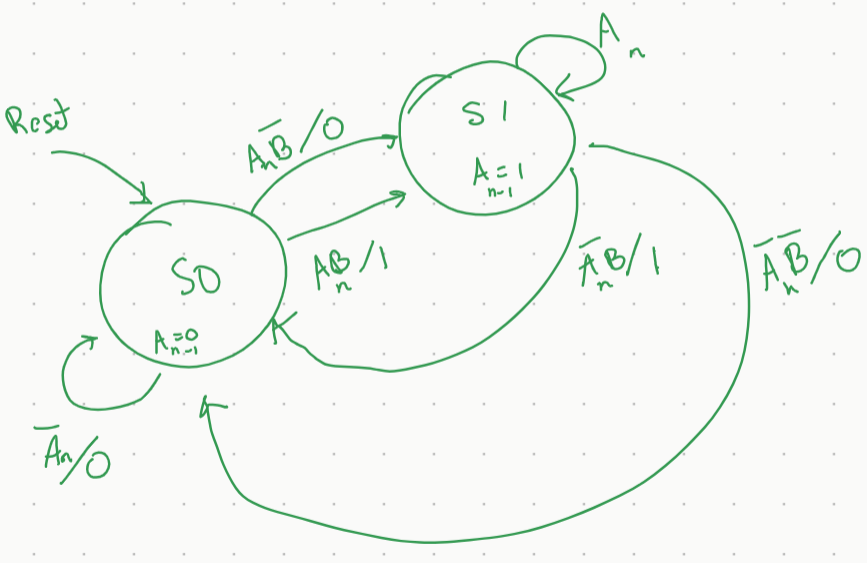
\includegraphics[width=0.6\textwidth]{03-29-state-machine}
			\caption{Mealy State machine for Exercise 3.29 (c)}
			\label{03-29-state-machine}
		\end{figure}
	\end{enumerate}
\end{sol}

\begin{ex}{3.30}
	Design an FSM with one input, $A$, and two outputs, $X$ and $Y$. $X$ should be 1
	if $A$ has been 1 for at least three cycles altogether (not necessarily consecutively).
	$Y$ should be 1 if $A$ has been 1 for at least two consecutive cycles.
	Show your state transition diagram, encoded state transition table, next state
	and output equations, and schematic.
\end{ex}

\begin{sol}
	See Figure~\ref{03-30-factored-state-machine}.
	\begin{figure}
		\centering
		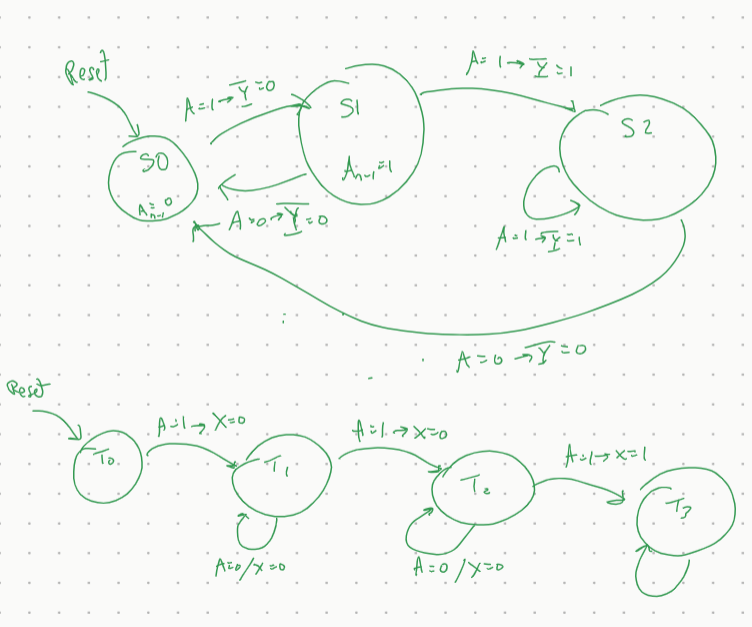
\includegraphics[width=0.6\textwidth]{03-30-factored-state-machine}
		\caption{Factored State Machine for Exercise 3.30}
		\label{03-30-factored-state-machine}
	\end{figure}
	The FSM has been written as a factored state machine. The topmost tracks controls
	the output $Y$, and the bottom one controls the output $X$.
\end{sol}

\begin{ex}{3.31}
	Analyze the FSM shown in Figure~\ref{03-31-circuit}.
	Write the state transition and output tables and sketch
	the state transition diagram.
	\begin{figure}
		\centering
		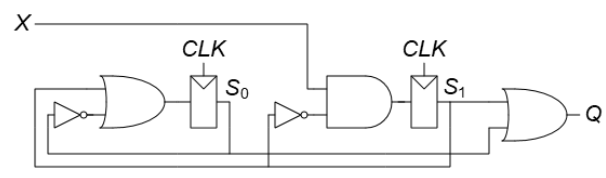
\includegraphics[width=0.6\textwidth]{03-31-circuit}
		\caption{FSM Schematic for Exercise 3.31}
		\label{03-31-circuit}
	\end{figure}
\end{ex}

\begin{sol}
	There are two state bits: $S_0$ and $S_1$. There
	is a single input $X$. We see from the circuit that:
	\begin{align*}
		S_1'&=X\bar{S_1}\\
		S_0'&=S1+\bar{S_0}\\
		Q&=S_1+S_0
	\end{align*}
	From these we can create next state and output tables:
	\begin{center}
		\begin{tabular}{cc|c|cc}
			$S_1$ & $S_0$ & $X$ & $S_1'$ & $S_0'$\\
			\hline
			0 & 0 & 0 & 0 & 1 \\
			0 & 0 & 1 & 1 & 1 \\
			0 & 1 & 0 & 0 & 0 \\
			0 & 1 & 1 & 1 & 0 \\
			1 & 0 & 0 & 0 & 1 \\
			1 & 0 & 1 & 0 & 1 \\
			1 & 1 & 0 & 0 & 1 \\
			1 & 1 & 1 & 0 & 1 \\
		\end{tabular}
		\quad
		\begin{tabular}{cc|c}
			$S_1$ & $S_0$ & $Q$\\
			\hline
			0 & 0 & 0\\
			0 & 1 & 1\\
			1 & 0 & 1\\
			1 & 1 & 1\\
		\end{tabular}
	\end{center}
	All states are reachable. Therefore, there are four states:
	\begin{center}
		\begin{tabular}{c|c}
			State & Encoding\\
			\hline
			$S0$ & $00$\\
			$S1$ & $01$\\
			$S2$ & $10$\\
			$S3$ & $11$\\
		\end{tabular}
	\end{center}
	The next state and output table is below in terms of the state names assigned above:
	\begin{center}
		\begin{tabular}{ccc}
			Current State & $X$ & New State \\
			\hline
			S0 & 0 & S1\\
			S0 & 1 & S3\\
			S1 & 0 & S0\\
			S1 & 1 & S2\\
			S2 & X & S1\\
			S3 & X & S1
		\end{tabular}
		\quad
		\begin{tabular}{c|c}
		State & $Q$\\
		\hline
		S0 & 0\\
		S1 & 1\\
		S2 & 1\\
		S3 & 1
		\end{tabular}
	\end{center}
	The state transition diagram is in Figure~\ref{03-31-state-transition-diagram}.
	\begin{figure}
		\centering
		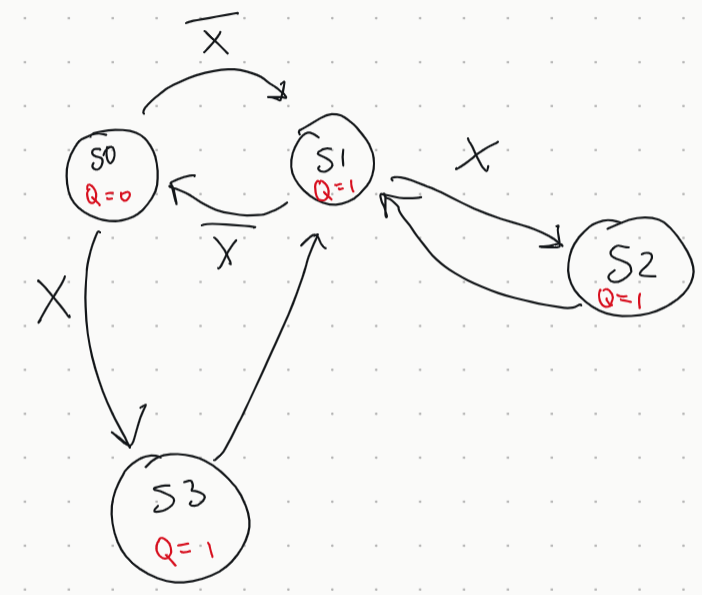
\includegraphics[width=0.6\textwidth]{03-31-state-transition-diagram}
		\caption{State transition diagram for Exercise 03-31}
		\label{03-31-state-transition-diagram}
	\end{figure}
\end{sol}

\begin{ex}{3.32}
	Repeat Exercise 3.31 for the FSM shown in Figure~\ref{03-32-circuit}. Recall that $s$ and
	$r$ register inputs indicate set and reset,
	respectively.
	\begin{figure}
		\centering
		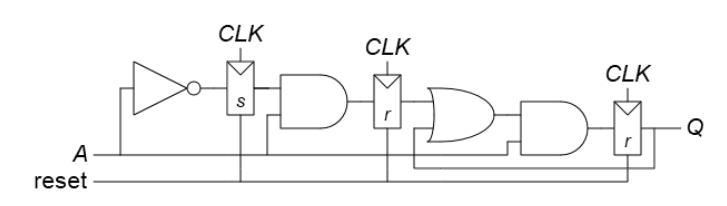
\includegraphics[width=0.6\textwidth]{03-32-circuit}
		\caption{FSM Schematic for Exercise 3.32}
		\label{03-32-circuit}
	\end{figure}
\end{ex}

\begin{sol}
	There are two resettable D flip-flops and 1 settable
	D flip-flop, so there are three state bits: $S_2$, $S_1$,
	and $S_0$.
	\begin{align*}
		S_2'&=\bar{A}\\
		S_1'&=S_2A\\
		S_0'&=(S_1+S_0)A\\
		Q&=S_0
	\end{align*}
	The next state and output tables are below:
	\begin{center}
		\begin{tabular}{ccc|c|ccc}
			$S_2$ & $S_1$ & $S_0$ & $A$ & $S_2'$ & $S_1'$ & $S_0'$\\
			\hline
			$0$ & $0$ & $0$ & $0$ & $1$ & $0$ & $0$\\
			$0$ & $0$ & $0$ & $1$ & $0$ & $0$ & $0$\\
			$0$ & $0$ & $1$ & $0$ & $1$ & $0$ & $0$\\
			$0$ & $0$ & $1$ & $1$ & $0$ & $0$ & $1$\\
			$0$ & $1$ & $0$ & $0$ & $1$ & $0$ & $0$\\
			$0$ & $1$ & $0$ & $1$ & $0$ & $0$ & $1$\\
			$0$ & $1$ & $1$ & $0$ & $1$ & $0$ & $0$\\
			$0$ & $1$ & $1$ & $1$ & $0$ & $0$ & $1$\\
			$1$ & $0$ & $0$ & $0$ & $1$ & $0$ & $0$\\
			$1$ & $0$ & $0$ & $1$ & $0$ & $1$ & $0$\\
			$1$ & $0$ & $1$ & $0$ & $1$ & $0$ & $0$\\
			$1$ & $0$ & $1$ & $1$ & $0$ & $1$ & $1$\\
			$1$ & $1$ & $0$ & $0$ & $1$ & $0$ & $0$\\
			$1$ & $1$ & $0$ & $1$ & $0$ & $1$ & $1$\\
			$1$ & $1$ & $1$ & $0$ & $1$ & $0$ & $0$\\
			$1$ & $1$ & $1$ & $1$ & $0$ & $1$ & $1$\\
		\end{tabular}
		\quad
		\begin{tabular}{ccc|c}
			$S_2$ & $S_1$ & $S_0$ & $Q$\\
			\hline
			$X$ & $X$ & $0$ & $0$\\
			$X$ & $X$ & $1$ & $1$\\
		\end{tabular}
	\end{center}
	Note that states $101$, $110$, and $111$ are not reachable, so we can
	eliminate them from the states table. Moreover, the only way to reach
	state $000$ is from itself, and the schematic indicates when
	reset is HIGH, the state bits are $S_2S_1S_0=100$. In other words,
	the system will never have a state of $000$. We use this to assign states
	and reduce the table:
	\begin{center}
		\begin{tabular}{ccc|c|ccc}
			$S_2$ & $S_1$ & $S_0$ & $A$ & $S_2'$ & $S_1'$ & $S_0'$\\
			\hline
			$0$ & $0$ & $1$ & $0$ & $1$ & $0$ & $0$\\
			$0$ & $0$ & $1$ & $1$ & $0$ & $0$ & $1$\\
			$0$ & $1$ & $0$ & $0$ & $1$ & $0$ & $0$\\
			$0$ & $1$ & $0$ & $1$ & $0$ & $0$ & $1$\\
			$0$ & $1$ & $1$ & $0$ & $1$ & $0$ & $0$\\
			$0$ & $1$ & $1$ & $1$ & $0$ & $0$ & $1$\\
			$1$ & $0$ & $0$ & $0$ & $1$ & $0$ & $0$\\
			$1$ & $0$ & $0$ & $1$ & $0$ & $1$ & $0$\\
		\end{tabular}
		\quad
		\begin{tabular}{c|c}
			State & Encoding\\
			\hline
			$S0$ & 001\\
			$S1$ & 010\\
			$S2$ & 011\\
			$S3$ & 100\\
		\end{tabular}
	\end{center}
	Using the new labels, the state transition and output tables are:
	\begin{center}
		\begin{tabular}{c|c|c}
			Current State & $A$ & New State\\
			\hline
			X & 0 & S3\\
			S0 & 1 & S0\\
			S1 & 1 & S0\\
			S2 & 1 & S0\\
			S3 & 1 & S1
		\end{tabular}
		\quad
		\begin{tabular}{c|c}
			State & $Q$\\
			\hline
			$S_0$ & $1$\\
			$S_1$ & $0$\\
			$S_2$ & $1$\\
			$S_3$ & $0$\\
		\end{tabular}
	\end{center}
	The state transition diagram for the circuit is given in Figure~\ref{03-32-state-transition-diagram}.
	\begin{figure}
		\centering
		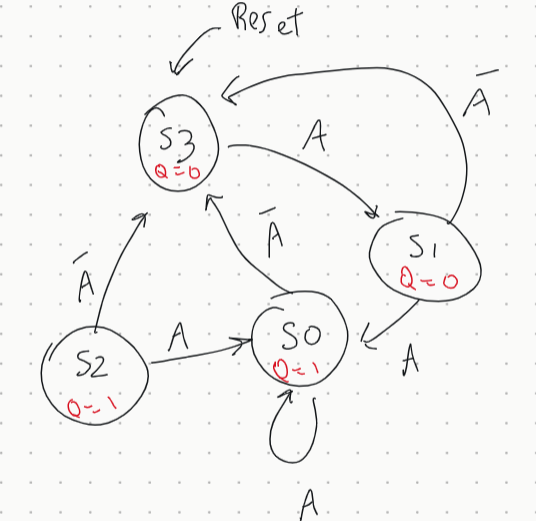
\includegraphics[width=0.5\textwidth]{03-32-state-transition-diagram}
		\caption{State transition diagram for Exercise 03-32}
		\label{03-32-state-transition-diagram}
	\end{figure}
\end{sol}

\begin{ex}{3.33}
	Ben Bitdiddle has designed the circuit in Figure~\ref{03-33-circuit} to compute a registered
	four-input XOR function. Each two-input XOR gate has a propagation delay of
	100 ps and a contamination delay of 55ps. Each flip-flop has a setup time
	of 60 ps, a hold time of 20 ps, a clock-to-$Q$ contamination maximum of 70 ps,
	and a clock-to-$Q$ minimum delay of 50 ps.
	\begin{enumerate}[label=(\alph*)]
		\item If there is no clock skew, what is the maximum operating frequency
		of the circuit?
		\item How much clock skew can the circuit tolerate if it must operate at
		2 GHZ?
		\item How much clock skew can the circuit tolerate before it might experience
		a hold time violation?
		\item Alyssa P. Hacker points out that she can resign the combinational
		logic between the registers to be faster \emph{and} tolerate more clock
		skew. Her improved circuit uses three two-input XORs, but they are arranged
		differently. What is her circuit? What is its maximum frequency if there
		is no clock skew? How much clock skew can the circuit tolerate before it might
		experience a hold time violation?
	\end{enumerate}
	\begin{figure}
		\centering
		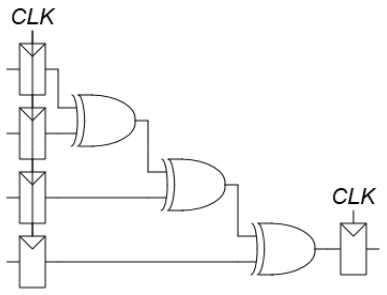
\includegraphics[width=0.4\textwidth]{03-33-circuit}
		\caption{Registered four-input XOR circuit for Exercise 3.33}
		\label{03-33-circuit}
	\end{figure}
\end{ex}

\begin{sol}
	\begin{enumerate}[label=(\alph*)]
		\item The maximum operating frequency $f_{c, max}$ corresponds to the smallest
		clock period or cycle time $T_{c, min}$. Recall that in the absence of
		clock skew, the period is given by:
		\[
		T_c\geq t_{pcd}+t_{pd}+t_{setup}=T_{c, min}
		\]
		Note $t_{pcd}$ is the maximum clock-to-$Q$ delay, so in this problem
		we have $t_{pcd}=70$ ps. Recall that the propagation delay through
		a comabinational circuit is the maximum time from when any input changes until
		all outputs reach their final value. Since the critical path goes through 3 XOR gates,
		this means that the propagation delay of the combinational logic is 3
		times the combinational delay of any one XOR gate. Lastly, keeping in mind
		that 1 ps = $10^{-12}$ s, we have:
		\[
		f_{c, max}=\frac{1}{T_{c, min}}=\frac{1}{70+3\cdot 100+60}\cdot 10^{-12} \text{Hz}
		=2.33\cdot 10^{9}\text{Hz}=2.33 \text{GHz}
		\]
		\item In the presence of clock skew, the clock period is given by:
		\[
		T_c > t_{pcd}+t_{pd}+t_{setup}+t_{skew}
		\]
		A frequency of $2$ GHz corresponds to a period of $T=\frac{1}{2\text{GHz}}=0.5$ ns,
		or 500 ps. We solve for $t_{skew}$:
		\[
		500> 70+300+60+t_{skew}\quad\implies\quad 70> t_{skew}
		\]
		Hence, it would tolerate a clock skew of at most 70 ps.
		\item In the presence of clock skew, we have:
		\[
		t_{ccq}+t_{cd}> t_{hold}+t_{skew}
		\]
		The question indicates that the minimum clock-to-$Q$ delay is 50 ps, so
		$t_{ccq}=50$ ps. Since the contamination delay of a combinational circuit is
		the minimum time from when any input changes until \emph{any} output
		starts to change its value, it follows that the contamination delay
		of the circuit is the contamination delay of any one XOR gate, or $t_{cd}=55$ ps.
		\[
		50+ 55> 20+t_{skew}
		\]
		Hence, $t_{skew}$ can be at most 85 ps.
		\item While Ben's XOR gates are arranged serially, Alyssa's XOR gates
		are arranged in parallel. See Figure~\ref{03-33-alyssa-circuit}.
		\begin{figure}
			\centering
			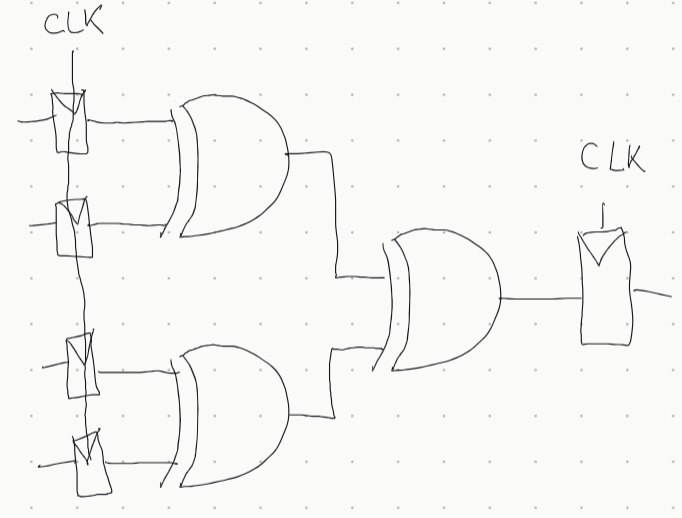
\includegraphics[width=0.5\textwidth]{03-33-alyssa-circuit}
			\caption{Alyssa's improved circuit for Exercise 3-33}
			\label{03-33-alyssa-circuit}
		\end{figure}
		Since the critical path in Alyssa's circuit goes through only 2 XOR gates,
		so the propagation delay is now 200 ps. Therefore,
		\[
		f_{c, max}=\frac{1}{T_{c, min}}=\frac{1}{70+2\cdot 100+60}\cdot 10^{-12} \text{Hz}
		=3.03\cdot 10^{9}\text{Hz}=3.03 \text{GHz}
		\]
		Meanwhile, the short path goes through 2 XOR gates also, so the contamination delay is $2\cdot 55$ ps=$110$ ps, so:
		\[
		50+110\geq 20+t_{skew}
		\]
		Hence, the circuit can tolerate 140 ps of clock skew before it might experience
		a hold time violation.
	\end{enumerate}
\end{sol}

\begin{ex}{3.34}
	You are designing an adder for the blindingly fast 2-bit RePentium Processor.
	The adder is built from two full adders, such that the carry out of the first adder
	is the carry in to the second adder, as shown in Figure~\ref{03-34-2-bit-adder-circuit}.
	
	\begin{figure}
		\centering
		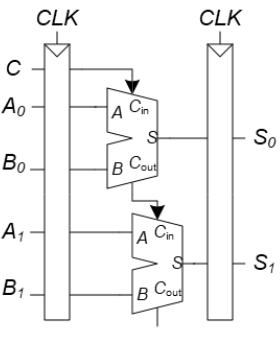
\includegraphics[width=0.3\textwidth]{03-34-circuit}
		\caption{2-bit adder schematic for Exercise 3.34}
		\label{03-34-2-bit-adder-circuit}
	\end{figure}
	
	Your adder has input and output registers and must complete the addition in one
	clock cycle. Each full adder has the following propagation delays: 20 ps from
	$C_{in}$ to $C_{out}$, or to \emph{Sum} ($S$), 25 ps from $A$ or $B$ to
	$C_{out}$, and 30 ps from $A$ or $B$ to $S$. The adder has a contamination delay
	of 15 ps from $C_{in}$ to either output and 2 ps from $A$ or $B$ to either output.
	Each flip-flop has a setup time of 30 ps, a hold time of 10 ps, a clock-to-$Q$
	propagation delay of 35 ps, and a clock-to-$Q$ contamination delay of $21$ ps.
	\begin{enumerate}[label=(\alph*)]
		\item If there is no clock skew, what is the maximum operating frequency of the circuit?
		\item How much clock skew can the circuit tolerate if it must operate at 8 GHz?
		\item How much clock skew can the circuit tolerate before it might experience a
		hold time violation?
	\end{enumerate}
\end{ex}

\begin{sol}
	\begin{enumerate}[label=(\alph*)]
		\item According to Figure 2.5 on Section 2.1, the functional specification of
		a full adder is:
		\begin{align*}
			S&=A\oplus B\oplus C_{in}\\
			C_{out}&=AB+AC_{in}+BC_{in}
		\end{align*}
		Hence, $S$ and $C_{out}$ are two outputs of each adder. The propagation
		delay through the first adder is the dictated by longest delay due to its
		input, which is 25 ps due to $A$ or $B$. This becomes
		$C_{in}$ for the second adder, for an additional 20 ps to settle in the second
		adder. In the absence of clock skew, the total propagation delay
		through both adders is 45 ps, and the maximum operating frequency of the circuit
		is
		\[
		f_{c, max}=\frac{1}{T_{c, min}}=
			\frac{1}{35+45+30}\text{ Hz}=9.09\text{ GHz}
		\]
		\item In order to operate at a minimum of 8 GHz, the maximum value of the clock
		period should be $T_{c}=\frac{1}{8\text{ GHz}}=125$ ps. Therefore, the
		maximum clock skew for it to operate at the desired frequency is given by:
		\[
		T_{c}> t_{pcd}+t_{pd}+t_{setup}+t_{skew}\quad\implies\quad 125> 35+45+30+t_{skew}
		\]
		or $t_{skew}< 15$ ps.
		\item The contamination delay of the circuit is $t_{cd}=15$ ps, because
		when $C_{in}$ begins to change in the first adder $C_{out}$ becomes to
		change in it as well, and hence $C_{in}$ begins to change in the second adder.
		Since $t_{ccq}=21$ ps and $t_{hold}=10$ ps, the maximum clock
		skew before it may experience a hold time violation is given by:
		\[
		t_{ccq}+t_{cd}> t_{hold}+t_{skew}\quad\implies\quad 21+15>10+t_{skew}
		\]
		or $t_{skew}<26$ ps.
	\end{enumerate}
\end{sol}

\begin{ex}{3.35}
	A \emph{field programmable gate array} (FGPA) uses \emph{configurable logic blocks (CLBs)}
	rather than logic gate to implement combinational logic. The Xilinx Spartan 3 FPGA
	has propagation and contamination delays of 0.61 and 0.30 ns, respectively, for each
	CLB. It also contains flip-flops with propagation and contamination delays of 0.72
	and 0.50 ns, and setup and hold times of 0.50 and 0 ns, respectively.
	\begin{enumerate}[label=(\alph*)]
		\item If you are building a system that needs to run at 40 MHz, how many
		consecutive CLBs can you use between two flip-flops? Assume that
		there is no clock skew and no delay through wires between CLBs.
		\item Suppose that all paths between flip-flops
		pass through at least one CLB. How much clock skew can the FPGA have
		without violating the hold time?
	\end{enumerate}
\end{ex}

\begin{sol}
	\begin{enumerate}[label=(\alph*)]
		\item In order to have at minimum clock frequency of 40 MHz, we need a maximum
		clock period of $T_{c}=\frac{1}{40\text{ MHz}}=25\cdot 10^{-9}\text { s}=25\text{ ns}$.
		Since the CLBs are placed consecutively (i.e., in series), the total
		propagation delay due to them is $t_{pd}=x\cdot 0.61$ ns, where $x$ is the number
		of CLBs. Hence,
		\[
		T_{c} \geq t_{pcd}+t_{pd}+t_{setup}\quad\implies\quad 25\geq0.72+0.61x+0.50\quad\implies\quad
		38.98\geq x
		\]
		Since $x$ is an integer, we allow at most 38 CLBs.
		\item Assuming $t_{cd}=0.30$ ns, which is the contamination delay through
		one CLB, then the maximum allowable clock skew is:
		\[
		t_{ccq}+t_{cd}> t_{hold}+t_{skew}\quad\implies\quad 0.50+0.3>0+t_{skew}
		\]
		or $t_{skew}<0.8$ ps or $800$ ns.
	\end{enumerate}
\end{sol}

\begin{ex}{3.36}
	A synchronizer is built from a pair of flip-flops with $t_{setup}=50$ ps,  $T_0=20$ ps,
	and $\tau=30$ ps. It samples an asynchronous input that changes $10^8$ times per second.
	What is the minimum clock period of the synchronizer to achieve a mean time between
	failures (MTBF) of 100 years?
\end{ex}

\begin{sol}
	The mean time between failures is given by
	\[
	\text{MTBF}=\frac{T_ce^{\frac{T_c-t_{\text{setup}}}{\tau}}}{NT_0}
	\]
	We are given $N=10^8$ Hz.  Since 100 years is $\approx \pi\times 10^{9}$ seconds, we get:
	\[
	\pi\times 10^{9}=\frac{T_ce^{\frac{T_c-50\cdot 10^{-12}}{30\cdot 10^{-12}}}}{10^{8}\cdot 20\cdot 10^{-12}}\quad\implies\quad
	2\pi\times 10^{6}=T_ce^{\frac{T_c-50\cdot 10^{-12}}{30\cdot 10^{-12}}}
	\]
	The solution is $T_c\approx 1.14\cdot 10^{-9}$ s, or $1.14$ ns.
\end{sol}

\end{document}